%%%%%%%%%%%%%%%%%%%%%%%%%%%%%%%%%%%%%%%%%
% Lab Report 2
% CS545_MachineLearning
% (2016SoE009)
%
%%%%%%%%%%%%%%%%%%%%%%%%%%%%%%%%%%%%%%%%%
%----------------------------------------------------------------------------------------
%	PACKAGES AND OTHER DOCUMENT CONFIGURATIONS
%----------------------------------------------------------------------------------------

\documentclass[12pt]{article}

\usepackage{fancyhdr} % Required for custom headers
\usepackage{lastpage} % Required to determine the last page for the footer
\usepackage{extramarks} % Required for headers and footers
\usepackage{graphicx} % Required to insert images
\usepackage{hyperref}
\usepackage{amsmath}
\usepackage{amsthm}
\usepackage{amssymb}
\usepackage{apacite}
\usepackage[english]{babel}
\usepackage{comment}
\usepackage{tikz}
\usetikzlibrary{shapes, arrows, positioning}
\tikzset{
    events/.style={ellipse, draw, align=right},
}

% paragraph indent
\newenvironment{myindentpar}[1]%
   {\begin{list}{}%
       {\setlength{\leftmargin}{#1}}%
           \item[]%
   }
     {\end{list}}

% Margins
\topmargin= -0.25in
\evensidemargin=0in
\oddsidemargin=0in
\textwidth=6.95in
\textheight=9.0in
\headsep=0.15in %distance between header and text

\linespread{1.2} % Line spacing

% Set up the header and footer
\pagestyle{fancy}
\lhead{Hwk \#2} % Top left header
\chead{CS 545 (M. Mitchell)} % Top center header
\rhead{bmarron} % Top right header
\lfoot{\lastxmark} % Bottom left footer
\cfoot{} % Bottom center footer
\rfoot{Page\ \thepage\ of\ \pageref{LastPage}} % Bottom right footer
\renewcommand\headrulewidth{0.4pt} % Size of the header rule
\renewcommand\footrulewidth{0.4pt} % Size of the footer rule

\setlength\parindent{0pt} % Removes all indentation from paragraphs
\setcounter{secnumdepth}{0} % Removes default section numbers

   
%----------------------------------------------------------------------------------------
%	NAME AND CLASS SECTION
%----------------------------------------------------------------------------------------

\newcommand{\hmwkClass}{Machine Learning (CS 545), Portland State University, Winter 2016} % Course/class
\newcommand{\hmwkTitle}{A Neural Network for Letter Recognition} % Assignment title
\newcommand{\hmwkAuthorName}{Bruce Marron} % Your name
\newcommand{\hmwkClassInstructor}{Mitchell} % Teacher/lecturer

%----------------------------------------------------------------------------------------
%	TITLE PAGE
%----------------------------------------------------------------------------------------

\title{
\vspace{2in}
\textmd{\textbf{\hmwkTitle}}\\
\textit{\normalsize \hmwkClass}
\vspace{3in}
}
\author{\textbf{\hmwkAuthorName}}
\date{2 February 2016} % Insert date here if you want it to appear below your name




%----------------------------------------
%	BEGIN DOC
%----------------------------------------
\begin{document}
\maketitle
\thispagestyle{empty}
\clearpage\maketitle

\subsection{Introduction}
A three-layer neural network was built in Python for the task of letter recognition from the Letter Recognition dataset, a publicly-available dataset from the UCI machine learning repository (https://archive.ics.uci.edu/ml/datasets/Letter+Recognition). The constructed neural network (\verb|Marron_NN1a.py|) draws heavily on the example given by \citeA{nielsen_neural_2015} but is distinct in its methods and attributes: there are no mini-batches, momentum has been added to the backpropagation algorithm, and most of Nielsen's original code has been parsed out to simpler statements.\footnote{Having no previous experience with Python, the author reverse-engineered Nielsen's code supplemented with numerous calls to the StackOverflow Exchange board in order to generate the neural network for this homework assignment.}\\

For the experiments outlined below, the neural network (\verb|Marron_NN1a.py|) was trained using a processed dataset of 10,000 entries (\verb|tr_d.pkl|) derived from the UCI dataset of 20,000 entries. Processing of the training dataset included standardization and the definition of a 26-dimensional target vector for each datum where the values for each target vector were set at 0.90 for the vector index corresponding to the correct English letter index (1-26) and to 0.10 otherwise.  The methodologies used for processing the training dataset are detailed in \verb|TrainingData_PreProcessing.txt|. A processed test dataset of 10,000 entries, the remaining entries from the UCI repository, was used to evaluate the network. This dataset was likewise standardized but using the mean and standard deviation values from the training dataset. The test dataset is available as (\verb|te_d.pkl|) and the details of processing are given in \verb|TestData_PreProcessing.txt|. Lastly, in every experiment the neural network was instantiated from a zero state (i.e., weights and biases set to zero) and optimized with stochastic gradient descent using the backpropagation algorithm. The neural network \verb|Marron_NN1a.py| applied the backpropagation algorithm in the following form,\\

\begin{align}
\frac{\partial E}{\partial b_{L3}} &= \nabla E_{L3} \odot \sigma'(z^{L3}) = \delta_{L3}\\
\frac{\partial E}{\partial w_{L3}} &= \delta_{L3}(a^{L2})^{T}\\
\frac{\partial E}{\partial b_{L2}} &= ((w_{L3})^T \delta_{L3}) \odot \sigma'(z^{L2}) = \delta_{L2}\\
\frac{\partial E}{\partial w_{L2}} &= \delta_{L2}(a^{L1})^{T}
\end{align}

where,
\begin{align*}
E &=  error \ function\\
b &= biases\\
w &= weights\\
L_i &= neural \ network \ layer \ counting \ from \ input \ to \ output, \ i = 1,2,3 \\
\odot  &= Hadamard \ operator\\
\sigma' &= the \ derivative \ of \ the \ sigmoid \ activation \ function, \frac{1}{1+e^{-z}}\\
z &= the \ raw \ network \ output \ per \ level\\
a &= the \ processed \ network \ output \ (activation) \ per \ level\\
T &= transpose
\end{align*}

\subsection{Experiment 1}
For this experiment, the network was trained for 100 epochs with a learning rate (eta) of 0.3, and a momentum factor (alpha) of 0.3. For each epoch, accuracy counts were recorded (1) on the training dataset (i.e., the accuracy of the network on the training dataset given the training dataset), and (2) on the test dataset (i.e., the accuracy of the network on the test dataset given the training dataset). The results of Experiment 1 are shown in Figure 1. 
\begin{figure}
  \begin{center}
    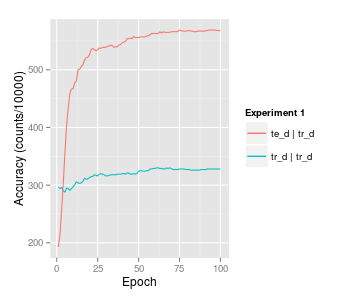
\includegraphics{Rplot1.png}
    \caption{The accuracy results for Experiment 1.}
  \end{center}
\end{figure}

\subsection{Experiment 2}
In this experiment, the network was trained for 100 epochs with a low learning rate ($\eta$ = 0.05) and a high learning rate ($\eta$ = 0.6) keeping the momentum rate constant ($\alpha$ = 0.3). For each epoch, accuracy counts were recorded (1) on the training dataset at low learning rate, (2) on the test dataset at low learning rate, (3) on the training dataset at high learning rate, and (4) on the test dataset at high learning rate. The results of Experiment 2 are shown in Figure 2.
\begin{figure}
  \begin{center}
    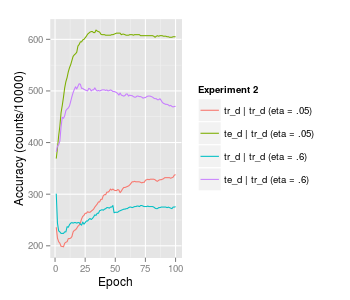
\includegraphics{Rplot2.png}
    \caption{The accuracy results for Experiment 2.}
  \end{center}
\end{figure}

\subsection{Experiment 3}
In this experiment, the network was trained for 100 epochs with a low momentum rate ($\alpha$ = 0.05) and a high momentum rate ($\alpha$ = 0.6) keeping the learning rate constant ($\eta$ = 0.3). For each epoch, accuracy counts were recorded (1) on the training dataset at low momentum rate, (2) on the test dataset at low momentum rate, (3) on the training dataset at high momentum rate, and (4) on the test dataset at high momentum rate. The results of Experiment 3 are shown in Figure 3.
\begin{figure}
  \begin{center}
    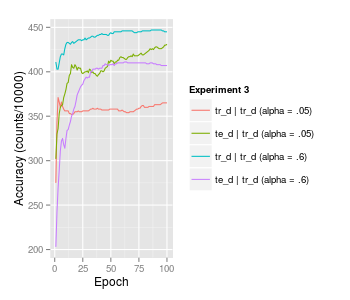
\includegraphics{Rplot3.png}
    \caption{The accuracy results for Experiment 3.}
  \end{center}
\end{figure}

\subsection{Experiment 4}
For the final experiment, the network itself was modified to contain two, rather than four, neurons in the hidden layer. Otherwise, Experiment 4 was identical to Experiment 1. The results of Experiment 4 are shown in Figure 4. 
\begin{figure}
  \begin{center}
    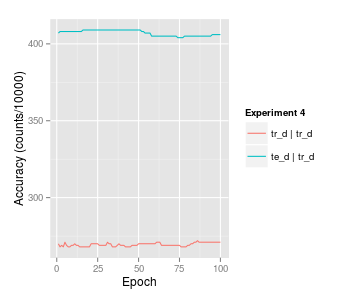
\includegraphics{Rplot4.png}
    \caption{The accuracy results for Experiment 4.}
  \end{center}
\end{figure}

\subsection{Results and Discussion}
Overall, the neural network defined in \verb|Marron_NN1a.py| performed poorly. This is most likely due to determinant error in the Python program since others have reported a 60\% accuracy or better.\footnote{Some fellow classmates reported greater than 60\% accuracy although others have been unable to break the 40\% mark.} Curiously, the network generally performed better on the test data than on the training data itself! It is suspected that there was somehow an imbalance in the selection of records for the training dataset when compared to the test dataset. Also, there were distinct differences in the effects of the learning parameter, $\eta $ and the momentum parameter, $\alpha $ as evidenced by performing the simple $2^{2}$ factorial experiment.

\subsection{Conclusions}
The backpropagation algorithm is a powerful and practical feedback cycle for machine learning. This algorithm appears to be a recent incarnation of the cybernetics, feedback-based approach to learning behavior \cite{ashby_introduction_1955, mackay_information_2003}. Perhaps relevant for an introductory class, duplication of results from well-tested networks could be included as part of the assignment in order to properly validate new programming code. A newly constructed neural network, in any programming language, should be able to generate the same outcomes as a well-tested network given identical initial conditions and optimization algorithms. Because neural networks appear to be sensitive to key parameters (here, learning rate, momentum rate, and the number of neurons in the hidden layer), the machine learning community undoubtedly has explored heuristics or perhaps analytical techniques for optimizing neural network performance. If not too complicated, these also might be incorporated as part of a neural network validation phase for the assignment.

\renewcommand{\refname}{\normalfont\selectfont\small \textbf{References}} 
\bibliographystyle{/usr/local/share/texmf/tex/latex/apacite/apacite}
\bibliography{/home/bmarron//Desktop/BibTex/2016SoE009}

\end{document}
